\section{质量的测量 \quad 天平}\label{sec:1-6}

在日常生活中我们可以看到许多称物体质量的工具。
比如在仓库和火车站可以看到能称很大质量的磅秤,
在商店可以看到使用方便的托盘秤和杆秤,
在药房和实验室可以看到能够精确地称质量的天平。
测量质量的工具很多,使用的时候,要根据需要适当地选用。

\begin{figure}[htbp]
    \centering
    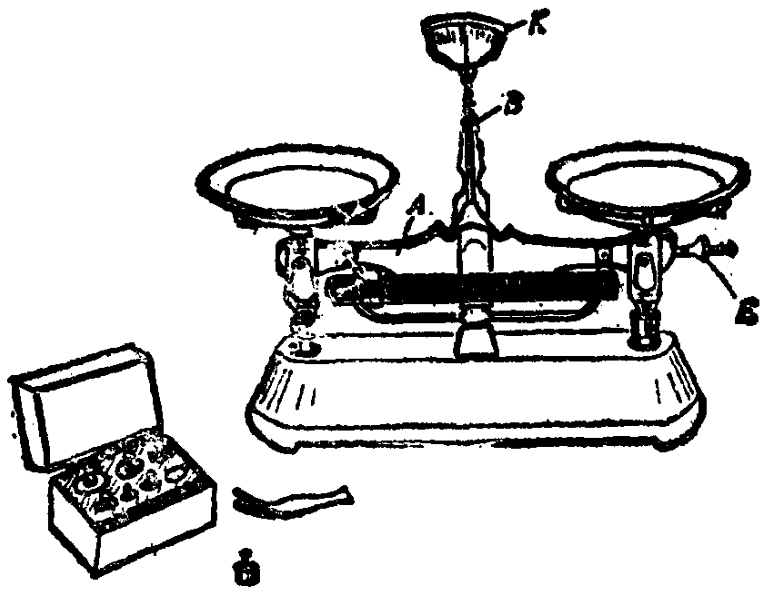
\includegraphics[width=0.6\textwidth]{../pic/czwl1-ch1-14}
    \caption{托盘天平和砝码}\label{fig:1-14}
\end{figure}

图 \ref{fig:1-14} 是实验室里常用的托盘天平。横梁 $A$ 可以自由摆动。
如果放在两个天平盘里的物体的质量不相等,质量较大的那端横梁就下沉。
\CJKunderwave{只有两个盘里的质量相等,横梁才停在水平位置,或者说横梁平衡了}。
天平就是根据这个道理来称物体质量的。

每架天平都配有一套砝码作为标准质量,装在砝码盒里,天平横梁上还附有标尺。
移动标尺上的游码相当于向天平盘里加小砝码。

使用托盘天平时,\CJKunderwave{应把天平放在水平桌面上}。
先把游码放在标尺左端的 “0” 点上,然后旋动横梁右端的调节螺母 $E$,
使指针 $B$ 对准刻度盘 $K$ 的中央,这就表示横梁平衡了。

测量的时候,把被测物体放在左盘里。估计被测物体的质量,选择适当的砝码放在右盘里。
如果右盘下沉,指针偏向刻度盘的右侧,这表示砝码的质量大了,可换用较小的砝码。
如果右盘上翘,指针偏向刻度盘左侧,就表示砝码的质量小了,可增加砝码,
并调节游码的位置,直到指针指在刻度盘的中央,横梁平衡为止。
这时盘里砝码的总质量加上游码所对的刻度值,就等于被测物体的质量。

天平是比较精密的仪器,使用要十分精心。
不要用手摸天平盘,更不准把潮湿的东西或化学药品直接放在天平盘里。
砝码要用镊子夹取,不准用手拿。
往盘里加减砝码要轻拿轻放,用后要及时放回砝码盒里,不要随意放置。
要注意保持天平和砝码干燥、清洁,防止锈蚀。
每架天平都有一定的称量范围,加在天平上的质量不能超过它的称量范围,否则会损伤天平。

